%% This file was auto-generated by IPython.
%% Conversion from the original notebook file:
%% kmeans.ipynb
%%
\documentclass[11pt,english,fleqn]{article}

%% This is the automatic preamble used by IPython.  Note that it does *not*
%% include a documentclass declaration, that is added at runtime to the overall
%% document.

\usepackage{amsmath}
\usepackage{amssymb}
\usepackage{graphicx}
\usepackage{ucs}
\usepackage[utf8x]{inputenc}

% needed for markdown enumerations to work
\usepackage{enumerate}

% Slightly bigger margins than the latex defaults
\usepackage{geometry}
\geometry{verbose,tmargin=3cm,bmargin=3cm,lmargin=2.5cm,rmargin=2.5cm}

% Define a few colors for use in code, links and cell shading
\usepackage{color}
\definecolor{orange}{cmyk}{0,0.4,0.8,0.2}
\definecolor{darkorange}{rgb}{.71,0.21,0.01}
\definecolor{darkgreen}{rgb}{.12,.54,.11}
\definecolor{myteal}{rgb}{.26, .44, .56}
\definecolor{gray}{gray}{0.45}
\definecolor{lightgray}{gray}{.95}
\definecolor{mediumgray}{gray}{.8}
\definecolor{inputbackground}{rgb}{.95, .95, .85}
\definecolor{outputbackground}{rgb}{.95, .95, .95}
\definecolor{traceback}{rgb}{1, .95, .95}

% Framed environments for code cells (inputs, outputs, errors, ...).  The
% various uses of \unskip (or not) at the end were fine-tuned by hand, so don't
% randomly change them unless you're sure of the effect it will have.
\usepackage{framed}

% remove extraneous vertical space in boxes
\setlength\fboxsep{0pt}

% codecell is the whole input+output set of blocks that a Code cell can
% generate.

% TODO: unfortunately, it seems that using a framed codecell environment breaks
% the ability of the frames inside of it to be broken across pages.  This
% causes at least the problem of having lots of empty space at the bottom of
% pages as new frames are moved to the next page, and if a single frame is too
% long to fit on a page, will completely stop latex from compiling the
% document.  So unless we figure out a solution to this, we'll have to instead
% leave the codecell env. as empty.  I'm keeping the original codecell
% definition here (a thin vertical bar) for reference, in case we find a
% solution to the page break issue.

%% \newenvironment{codecell}{%
%%     \def\FrameCommand{\color{mediumgray} \vrule width 1pt \hspace{5pt}}%
%%    \MakeFramed{\vspace{-0.5em}}}
%%  {\unskip\endMakeFramed}

% For now, make this a no-op...
\newenvironment{codecell}{}

 \newenvironment{codeinput}{%
   \def\FrameCommand{\colorbox{inputbackground}}%
   \MakeFramed{\advance\hsize-\width \FrameRestore}}
 {\unskip\endMakeFramed}

\newenvironment{codeoutput}{%
   \def\FrameCommand{\colorbox{outputbackground}}%
   \vspace{-1.4em}
   \MakeFramed{\advance\hsize-\width \FrameRestore}}
 {\unskip\medskip\endMakeFramed}

\newenvironment{traceback}{%
   \def\FrameCommand{\colorbox{traceback}}%
   \MakeFramed{\advance\hsize-\width \FrameRestore}}
 {\endMakeFramed}

% Use and configure listings package for nicely formatted code
\usepackage{listingsutf8}
\lstset{
  language=python,
  inputencoding=utf8x,
  extendedchars=\true,
  aboveskip=\smallskipamount,
  belowskip=\smallskipamount,
  xleftmargin=2mm,
  breaklines=true,
  basicstyle=\small \ttfamily,
  showstringspaces=false,
  keywordstyle=\color{blue}\bfseries,
  commentstyle=\color{myteal},
  stringstyle=\color{darkgreen},
  identifierstyle=\color{darkorange},
  columns=fullflexible,  % tighter character kerning, like verb
}

% The hyperref package gives us a pdf with properly built
% internal navigation ('pdf bookmarks' for the table of contents,
% internal cross-reference links, web links for URLs, etc.)
\usepackage{hyperref}
\hypersetup{
  breaklinks=true,  % so long urls are correctly broken across lines
  colorlinks=true,
  urlcolor=blue,
  linkcolor=darkorange,
  citecolor=darkgreen,
  }

% hardcode size of all verbatim environments to be a bit smaller
\makeatletter 
\g@addto@macro\@verbatim\small\topsep=0.5em\partopsep=0pt
\makeatother 

% Prevent overflowing lines due to urls and other hard-to-break entities.
\sloppy

\setlength{\mathindent}{0pt}
\setlength{\parindent}{0pt}
\setlength{\parskip}{8pt}
\begin{document}

K-Means Kumeleme Metodu

Yapay Ogrenim (Machine Learning) alaninda onemli algoritmalardan biri
k-means metodu. K-means kumelemesi icin kac tane kumenin olmasi
gerektigi bastan tanimlanir (yani k parametresi), algoritma bunu kendisi
bulmaz.

Metotun geri kalani basittir - bir dongu (iteration) icinde her
basamakta:

\begin{enumerate}[1)]
\item
  Her nokta icin, eldeki kume merkezleri teker teker kontrol edilir ve o
  nokta en yakin olan kumeye atanir
\item
  Atamalar tamamlandiktan sonra her kume icinde hangi noktalarin oldugu
  bilindigi icin her kumedeki noktalarin ortalamasi alinarak yeni kume
  merkezi hesaplanir. Eski merkez hesaplari atilir.
\item
  Basa donulur
\end{enumerate}
Dongu tekrar ilk adima dondugunde, bu sefer yeni kume merkezlerini
kullanilarak, ayni adimlar tekrar yapilacaktir.

Fakat bir problem yok mu? Daha birinci dongu baslamadan kume
merkezlerinin nerede oldugunu nereden bilecegiz? Burada bir
tavuk-yumurta problemi var, kume merkezleri olmadan noktalari
atayamayiz, atama olmadan kume merkezlerini hesaplayamayiz.

Bu probleme pratik bir cozum ilk basta kume merkezlerini (ya da kume
atamalarini) rasgele bir sekilde secmektir. Pratikte bu yontem cok iyi
isliyor. Tabii bu rasgelelik yuzunden K-means'in dogru sonuca yaklasmasi
(convergence) garanti degildir, ama gercek dunya uygulamalarinda
cogunlukla kullanisli kumeler bulunur. Bu potansiyel problemlerden
kacinmak icin k-means pek cok kez isletilebilir (her seferinde yeni
rasgele baslangiclarla yani) ve ayni sonuca ulasilip ulasilmadigi
kontrol edilebilir.

Pek en iyi k nasil bulunur? Burada da yapay ogrenim literaturunde pek
cok yaklasim vardir {[}1{]}, veriyi pek cok parcaya bolup, farkli k kume
sayisi icin kumeleme yapmak ve capraz saglama (cross-validation)
kullanmak, SVD kullanarak grafige bakmak (bu yazinin sonunda
anlatiliyor), vs.

K-Means EM algoritmasinin bir turevi olarak kabul edilebilir, EM
kumeleri bir Gaussian (ya da Gaussian karisimi) gibi gorur, ve her
basamakta bu dagilimlarin merkezini, hem de kovaryansini hesaplar. Yani
kumenin ``sekli'' de EM tarafindan saptanir. Ayrica EM her noktanin tum
kumelere olan uyeliklerini ``hafif (soft)'' olarak hesaplar (bir
olasilik olcutu uzerinden), fakat K-Means icin bu atama nihai (hard
membership). Nokta ya bir kumeye aittir, ya da degildir.

EM'in belli sartlarda yaklasiksalligi icin matematiksel ispat var.
K-Means akilli tahmin yaparak (heuristic) calisan bir algoritma olarak
biliniyor. Sonuca yaklasmasi bu sebeple garanti degildir, ama daha once
belirttigimiz gibi pratikte faydalidir. Bir suru alternatif kumeleme
yontemi olmasina ragmen hala K-Means'den vazgecilemiyor! Burada bir
etken de K-Means'in cok rahat paralelize edilebilmesi. Bu konu baska bir
yazida islenecek.

Ornek test verisi altta

\begin{codecell}
\begin{codeinput}
\begin{lstlisting}
from pandas import *
data = read_csv("synthetic.txt",names=['a','b'],sep="   ")
print data.shape
data = np.array(data)
\end{lstlisting}
\end{codeinput}
\begin{codeoutput}
\begin{verbatim}
(3000, 2)
\end{verbatim}
\end{codeoutput}
\end{codecell}
\begin{codecell}
\begin{codeinput}
\begin{lstlisting}
scatter(data[:,0],data[:,1])
\end{lstlisting}
\end{codeinput}
\begin{codeoutput}
\begin{verbatim}
<matplotlib.collections.PathCollection at 0x358d390>
\end{verbatim}
\begin{center}
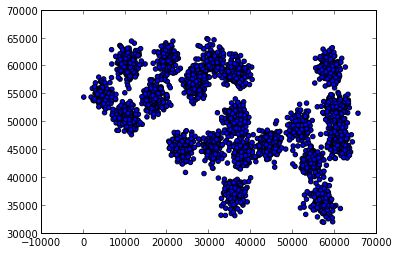
\includegraphics[width=0.7\textwidth]{kmeans_files/kmeans_fig_00.png}
\par
\end{center}
\end{codeoutput}
\end{codecell}
\begin{codecell}
\begin{codeinput}
\begin{lstlisting}
def euc_to_clusters(x,y):
    return np.sqrt(np.sum((x-y)**2, axis=1))

class KMeans():
    def __init__(self,k,iter):
        self.k = k
        self.iter = iter
    def fit(self,X):
        # her veri noktasi icin rasgele kume merkezi ata
        self.labels_ = np.array([random.randint(0,self.k-1) for i in range(X.shape[0])])
        self.centers_ = np.zeros((self.k,X.shape[1]))
        for i in range(self.iter):
            # yeni kume merkezleri uret
            for j in range(self.k):
                # eger kume j icinde hic nokta yoksa, ortalama (mean)
                # hesabi yapma, cunku o zaman nan degeri geliyor, ve
                # hesabin geri kalani bozuluyor.
                if len(X[self.labels_ == j]) == 0: continue
                center = np.mean(X[self.labels_ == j],axis=0)
                self.centers_[j,:] = center
            # her nokta icin kume merkezlerine gore kume atamasi yap
            self.labels_ = []
            for point in X:
                c = np.argmin(euc_to_clusters(self.centers_, point))
                self.labels_.append(int(c))

            self.labels_ = np.array(self.labels_)

\end{lstlisting}
\end{codeinput}
\end{codecell}
\begin{codecell}
\begin{codeinput}
\begin{lstlisting}
cf = KMeans(k=5,iter=20)
cf.fit(data)
cf.labels_
\end{lstlisting}
\end{codeinput}
\begin{codeoutput}
\begin{verbatim}
array([1, 1, 1, ..., 0, 0, 0])
\end{verbatim}
\end{codeoutput}
\end{codecell}
Ustteki sonucun icinde iki ana vektor var, bu vektorlerden birincisi
icinde 4,1, gibi sayilar goruluyor, bu sayilar her noktaya tekabul eden
kume atamalari. Ikinci vektor icinde iki boyutlu k tane vektor var, bu
vektorler de her kumenin merkez noktasi. Merkez noktalarini ham veri
uzerinde grafiklersek (kirmizi noktalar)

\begin{codecell}
\begin{codeinput}
\begin{lstlisting}
scatter(data[:,0],data[:,1])
plt.hold(True)
plt.ylim([30000,70000])
for x in cf.centers_: plot(x[0],x[1],'rd')
    
\end{lstlisting}
\end{codeinput}
\begin{codeoutput}
\begin{center}
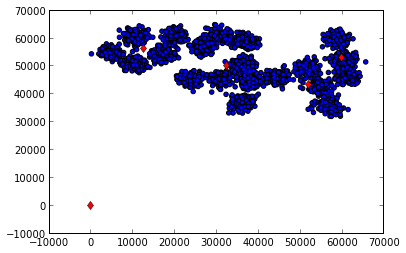
\includegraphics[width=0.7\textwidth]{kmeans_files/kmeans_fig_01.png}
\par
\end{center}
\end{codeoutput}
\end{codecell}
Goruldugu gibi 5 tane kume icin ustteki merkezler bulundu. Fena degil.
Eger 10 dersek

\begin{codecell}
\begin{codeinput}
\begin{lstlisting}
cf = KMeans(k=15,iter=20)
cf.fit(data)
scatter(data[:,0],data[:,1])
plt.ylim([30000,70000])
plt.hold(True)
for x in cf.centers_: plot(x[0],x[1],'rd')
\end{lstlisting}
\end{codeinput}
\begin{codeoutput}
\begin{center}
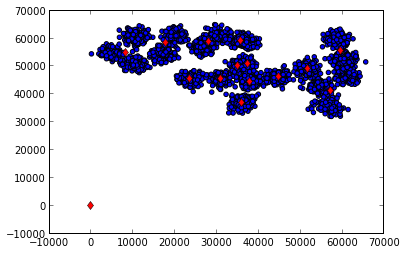
\includegraphics[width=0.7\textwidth]{kmeans_files/kmeans_fig_02.png}
\par
\end{center}
\end{codeoutput}
\end{codecell}
\subsection{Kategorik ve Numerik Iceren Karisik Veriler}

Bazen verimiz hem kategorik hem de numerik degerler iceriyor olabilir,
KMeans yeni kume merkezlerini hesaplarken ortalama operasyonu kullandigi
icin sadece numerik veriler uzerinde calisabilir (kategorik verilerin
nasil ortalamasini alalim ki?). Bu durumda ne yapacagiz?

Bir secenek su olabilir, kategorik her kolonu her degisik degeri bir
yeni kolona tekabul edecek sekilde saga dogru acariz, ve o degerin yeni
kolonuna 1 degeri digerlerine 0 degeri veririz. Bu kodlamaya 1-in-q
kodlamasi, 1-in-n kodlamasi, ya da Ingilizce one-hot encoding ismi
veriliyor.

Ornek olarak UCI veri bankasindan Avustralya Kredi Verisine bakalim:

\begin{codecell}
\begin{codeinput}
\begin{lstlisting}
import pandas as pd
df = pd.read_csv("crx.csv")
df[:2]
\end{lstlisting}
\end{codeinput}
\begin{codeoutput}
\begin{verbatim}
  A1     A2    A3 A4 A5 A6 A7    A8 A9 A10  A11 A12 A13    A14  A15 A16
0  b  30.83  0.00  u  g  w  v  1.25  t   t    1   f   g  00202    0   +
1  a  58.67  4.46  u  g  q  h  3.04  t   t    6   f   g  00043  560   +
\end{verbatim}
\end{codeoutput}
\end{codecell}
Bu veride A1, A2, gibi kolon isimleri var, kategorik olanlarda `g',`w'
gibi degerler goruluyor. Bu kolonlari degistirmek icin

\begin{codecell}
\begin{codeinput}
\begin{lstlisting}
from sklearn.feature_extraction import DictVectorizer
def one_hot_dataframe(data, cols, replace=False):
    vec = DictVectorizer()
    mkdict = lambda row: dict((col, row[col]) for col in cols)
    vecData = pd.DataFrame(vec.fit_transform(data[cols].apply(mkdict, axis=1)).toarray())
    vecData.columns = vec.get_feature_names()
    vecData.index = data.index
    if replace is True:
        data = data.drop(cols, axis=1)
        data = data.join(vecData)
    return (data, vecData, vec)

df2, _, _ = one_hot_dataframe(df, ['A1','A4','A5','A6','A7','A9','A10','A12','A13'], replace=True)
df2.ix[0]
\end{lstlisting}
\end{codeinput}
\begin{codeoutput}
\begin{verbatim}
A2       30.83
A3           0
A8        1.25
A11          1
A14      00202
A15          0
A16          +
A10=f        0
A10=t        1
A12=f        1
A12=t        0
A13=g        1
A13=p        0
A13=s        0
A1=?         0
A1=a         0
A1=b         1
A4=?         0
A4=l         0
A4=u         1
A4=y         0
A5=?         0
A5=g         1
A5=gg        0
A5=p         0
A6=?         0
A6=aa        0
A6=c         0
A6=cc        0
A6=d         0
A6=e         0
A6=ff        0
A6=i         0
A6=j         0
A6=k         0
A6=m         0
A6=q         0
A6=r         0
A6=w         1
A6=x         0
A7=?         0
A7=bb        0
A7=dd        0
A7=ff        0
A7=h         0
A7=j         0
A7=n         0
A7=o         0
A7=v         1
A7=z         0
A9=f         0
A9=t         1
Name: 0, Length: 52, dtype: object
\end{verbatim}
\end{codeoutput}
\end{codecell}
Islem sonucunda A12=f mesela icin 1 verilmis, ama A12=t (ve diger her
mumkun deger icin yani) 0 degeri verilmis (sadece bu tek satir icin).
Boylece kategorik veriyi sayisal hale cevirmis olduk.

Fakat isimiz bitti mi? Hayir. Simdi KMeans bu tur veriyle acaba duzgun
calisir miydi onu kendimize soralim. Icinde pek cok 0, bazen 1 iceren
veri satirlari arasinda uzaklik hesabi yapmak ise yarar mi?

Yapay Ogrenim literaturunde bu tur veriler uzerinde kosinus benzerligi
(cosine similarity) kullanmak daha yaygindir. Bu konuyu SVD, Toplu
Tavsiye yazinda daha gorebilirsiniz. Kosinus benzerligi bize 0 ile 1
arasinda bir deger dondurur. Benzerligi uzakliga cevirmek icin basit bir
sekilde 1-benzerlik formulunu kullanabiliriz.

O zaman karisik veriler uzerinde KMeans kullanmak icin sunu yapariz,
verinin en bastan numerik olan kismi icin Oklit uzakligi, diger kalan
kismi icin kosinus uzakligi kullaniriz.

\begin{codecell}
\begin{codeinput}
\begin{lstlisting}
from numpy import linalg as la
import numpy as np
import pandas as pd, os
import scipy.sparse as sps
import numpy, random

def cos_dist(inA,inB):
    num = float(np.dot(inA.T,inB))
    denom = la.norm(inA)*la.norm(inB)
    sim = 0.5+0.5*(num/denom)
    return 1. - sim

def mixed_to_clusters(vect,x,euc_n,weights):
    res1 = euc_to_clusters(vect[:,0:euc_n],x[0:euc_n])
    res2 = map(lambda y: cos_dist(x[euc_n:],y), vect[:,euc_n:])
    res = np.array(res1)*weights[0] + np.array(res2)*weights[1]
    return res

class MixedKMeans():
    def __init__(self,k,iter,euc_n,weights=[1.,1.]):
        self.k = k
        self.iter = iter
        self.euc_n = euc_n
        self.weights = weights
    def fit(self,X,iter=10):
        self.labels_ = np.array([random.randint(0,self.k-1) for i in range(X.shape[0])])
        self.centers_ = np.zeros((self.k,X.shape[1]))
        for i in range(self.iter):
            for j in range(self.k):
                if len(X[self.labels_ == j]) == 0: continue
                center = np.mean(X[self.labels_ == j],axis=0)
                self.centers_[j,:] = center
            self.labels_ = []
            for point in X:
                c = np.argmin(mixed_to_clusters(self.centers_, point, self.euc_n,self.weights))
                self.labels_.append(int(c))

            self.labels_ = np.array(self.labels_)

\end{lstlisting}
\end{codeinput}
\end{codecell}
\begin{codecell}
\begin{codeinput}
\begin{lstlisting}
df = pd.read_csv("crx.csv",sep=',',na_values=['?'])
df = df.dropna()

df['A16'] = df['A16'].str.replace('+','1')
df['A16'] = df['A16'].str.replace('-','0')
df['A16'] = df['A16'].astype(int)

df2, _, _ = one_hot_dataframe(df, ['A1','A4','A5','A6','A7','A9','A10','A12','A13'], replace=True)
df2 = df2.drop('A16',axis=1)

df2 = np.array(df2)

# veriyi normalize et, ortalama cikar ve standart sapmaya bol
df2 -= np.mean(df2, axis=0)
df2 /= np.std(df2, axis=0)

cf = MixedKMeans(2,iter=10,euc_n=6,weights=[1.,3.])
cf.fit(df2)

labels_true = np.array(df['A16'])
labels_pred = cf.labels_
match = np.sum((labels_true == labels_pred).astype(int))
print float(match)/len(df)   
\end{lstlisting}
\end{codeinput}
\begin{codeoutput}
\begin{verbatim}
0.814701378254
\end{verbatim}
\end{codeoutput}
\end{codecell}
Bu veri icinde iki tane kume vardi, kumeler A16 kolonunda + ya da -
olarak isaretli. Tabii kumeleme takip edilmeyen (unsupervised) bir Yapay
Ogrenim metotududur, hangi noktanin hangi kumeye ait oldugunu onceden
bilmeyiz, ornek veri seti uzerinde kontrol amacli bu isaretlere
bakiyoruz. Ustteki sonuca gore yuzde 81 oraninda bir basariyla dogru
kumeyi bulabilmisiz.

Parametre olarak gecilen euc\_n degiskeni her veri noktasi icin ``ilk
kac noktanin numerik'' oldugunu belirtiyor. Boylece uzaklik fonksiyonu
sadece o kisimda Oklit uzakligi kullaniyor. Peki numerik degerler niye
hep basta? Bunun sebebi one\_hot\_dataframe cagrisinin yeni kolonlari
yaratirken eskileri silmesi ve eklenen yeni kolonlarin hep en sona
konmasi, boylece en bastakiler hep numerik kolon oluyor!

Agirliklar

Oklit ve kosinus uzakliklarini birbirine toplarken, birine digerinden
daha fazla agirlik vermek mumkun, belki de bir veri seti icin numerik
veriler kategorik olanlardan daha onemli, bu durumda agirliklari, mesela
ustte 1'e 3 olarak tanimladik, Oklit uzakligina 3 kat daha fazla onem /
agirlik vermis oluruz (cunku kategorik verileri 3 kat daha
``fazlalastiriyoruz'', ``uzaklastiriyoruz''). Bu agirliklar tahmin,
deneme / yanilma, tecrube ile bulunmali, veri setine gore degisik
olacaklardir.

Normalize Etmek

Ustteki ornekte veriyi 1-in-n kodlamasiyla cevirdikten sonra bir de
normalize ettik, yani her kolon bazinda o kolonun ortalamasini o
kolondaki tum degerlerden cikarttik ve standart sapmaya bolduk, boylece
her kolonu 0 etrafinda ortalayip onun iki tarafina dusebilecek -/+
degerleri kucultuyoruz. Bu veriyi bir tur ``sekle sokma'' islemidir, ne
zaman kullanilacagi tecrubeyle ortaya cikar, mesela ustteki karisik
veride bunun isleyebilecegini tahmin ettik.

Kume sayisini bulmak

KMeans'e kume sayisinin onceden verilmis olmasi gerekiyor, ve bu sayiyi,
metot takip edilmeyen metot oldugu icin, bastan bilmiyoruz. Bu sayiyi
bir sekilde bulmanin yolu olamaz mi?

Eger boyut azaltma teknigi SVD'yi kullanirsak, bu mumkun olabilir. SVD
sonrasi elimize azaltilmis bir veri gececek, ve bu veride en basta olan
kolonlar en onemli olanlardir, ve bu kolonlari, mesela ilk ikisini
alarak ekrana basabiliriz. Avustralya Kredi setinde bunu yaparsak sunu
goruruz:

\begin{codecell}
\begin{codeinput}
\begin{lstlisting}
import scipy.linalg as lin
u,s,vt=lin.svd(df2) # normalize edilmis veri uzerinde
plt.plot(u[:,0], u[:,1],'.')

\end{lstlisting}
\end{codeinput}
\begin{codeoutput}
\begin{verbatim}
[<matplotlib.lines.Line2D at 0x46f4e90>]
\end{verbatim}
\begin{center}
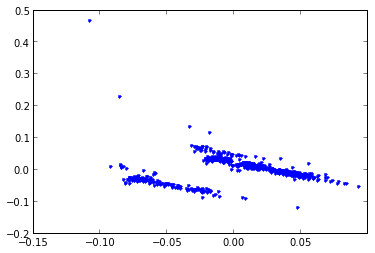
\includegraphics[width=0.7\textwidth]{kmeans_files/kmeans_fig_03.png}
\par
\end{center}
\end{codeoutput}
\end{codecell}
Iki tane ana blok oldugu acik bir sekilde goruluyor. Demek ki kume
sayisi k = 2 kullanmak gerekir.

Bazi ek notlar

{[}1{]}
http://en.wikipedia.org/wiki/Determining\_the\_number\_of\_clusters\_in\_a\_data\_set

{[}2{]}
nbviewer.ipython.org/url/cbcb.umd.edu/\ensuremath{\sim}hcorrada/PML/src/kmeans.ipynb

\end{document}
